\documentclass[margin=1mm]{standalone}
\usepackage{enumitem}
\usepackage[skip=3mm, indent=0mm]{parskip}
\usepackage{fontspec}
\setmainfont{QTHeidelbergType}

\usepackage[x11names]{xcolor}
\usepackage{tikz}
\colorlet{fascist}{OrangeRed1}
\colorlet{liberal}{Turquoise4}


\begin{document}
	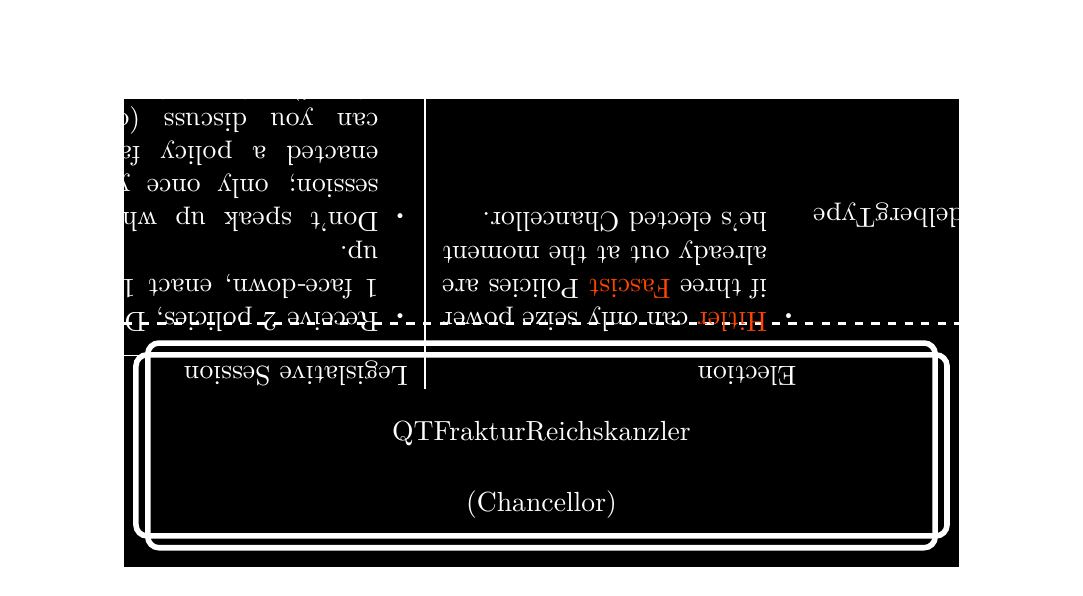
\begin{tikzpicture}		
		\fill (-5.3,-1.7) rectangle (5.3,4.1);
		
		\node at (0,0)[white] {\fontsize{40}{40}\setmainfont{QTFraktur}Reichskanzler};
		\node at (0,-0.9) [white] {(Chancellor)};
		
		\draw [white] [line width=2, rounded corners] (-5.15,1) rectangle (5.15,-1.3);
		\draw [white] [line width=2, rounded corners] (-5,1.15) rectangle (5,-1.45);
		
		\fill [black] (-5.3, 1.4) rectangle (5.3, 4.25);
		\draw [dashed, line width=1, white] (-5.3, 1.4)--(5.3, 1.4);
		\draw (-5.3, 1.7) rectangle (5.3, 4);
		
		\begin{scope}[yshift=2.8cm]
			\node at (0,0) [rotate=180,white] {\fontsize{6}{6}\setmainfont{QTHeidelbergType}\begin{tabular}{p{4.5cm}|p{4.5cm}}
					Election & Legislative Session\\
					\hline
					\begin{itemize}[leftmargin=*]
						\item \textcolor{fascist}{Hitler} can only seize power if three \textcolor{fascist}{Fascist} Policies are already out at the moment he's elected Chancellor.
					\end{itemize} & 
					\begin{itemize}[leftmargin=*]
						\item Receive 2 policies, Discard 1 face-down, enact 1 face-up.
						\item Don't speak up while in session; only once you've enacted a policy face-up can you discuss (or lie about!) what policies you were passed.
					\end{itemize}
			\end{tabular}};
		\end{scope}
		
	\end{tikzpicture}
\end{document}